\chapter{自由电子气} % (fold)
\label{cha:自由电子气}
\section{Introduction} % (fold)
\label{sec:Introduction 8}
电子是费米子,由于Pauli不相容原理,宏观量级的电子最终会排布到很高的能级上,这个能级我们就称之为费米能级\index{费米能级}。

金属中的自由电子我们依旧使用真空电子势箱模型来描述,因此电子的各个能级也就是真空势箱中自由粒子的平动能级。所以费米能级附近的粒子实际上具有相当高的动能。由于这些粒子的动能很大,电子和正离子、电子和电子之间的相互作用势能可以忽略,所以我们可以近似看出自由电子气。
% section Introduction (end)
\section{统计分析} % (fold)
\label{sec:统计分析}
对于费米子,我们使用Fermi-Dirac分布$f(\mu)$来描述其能量分布,这个分布函数的大概图像为
\begin{figure}[h]
       \centering
       \subfigure[正常温度情形]{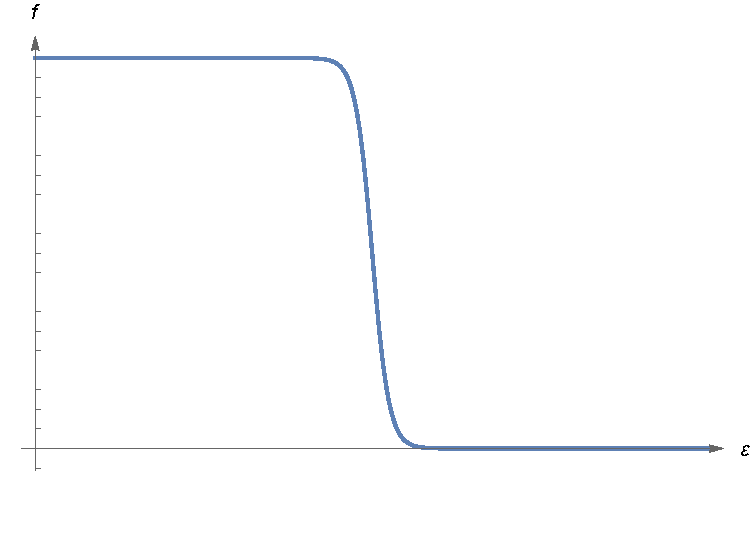
\includegraphics[width=0.42\textwidth]{fig/Fermi distribution.pdf}}\qquad
       \subfigure[低温情形]{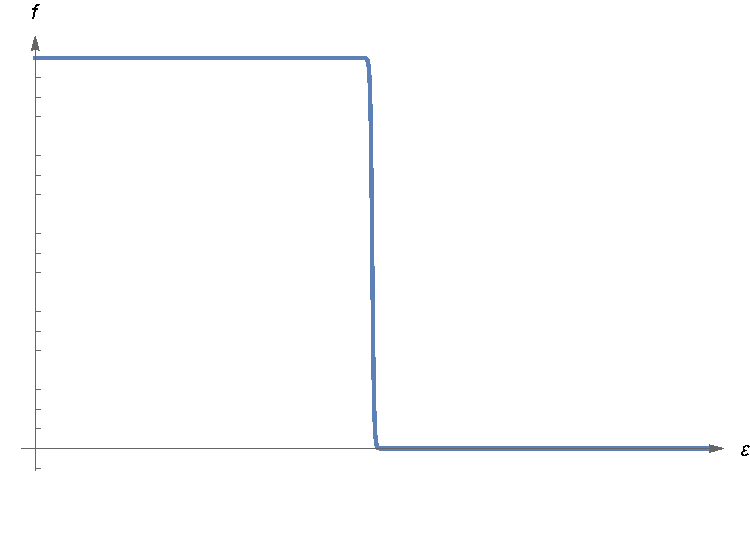
\includegraphics[width=0.42\textwidth]{fig/sharp fermidis.pdf}}
       \caption{Fermi-Dirac分布的大概图像}
       \label{fig:fermi distribution}
\end{figure}
而不同能级的总粒子数量满足满足关系\begin{equation}
    N(\varepsilon) = C \sqrt{\varepsilon} f(\varepsilon) 
\end{equation}
其图像为
\begin{figure}[h]
    \centering
    \subfigure[正常温度情形]{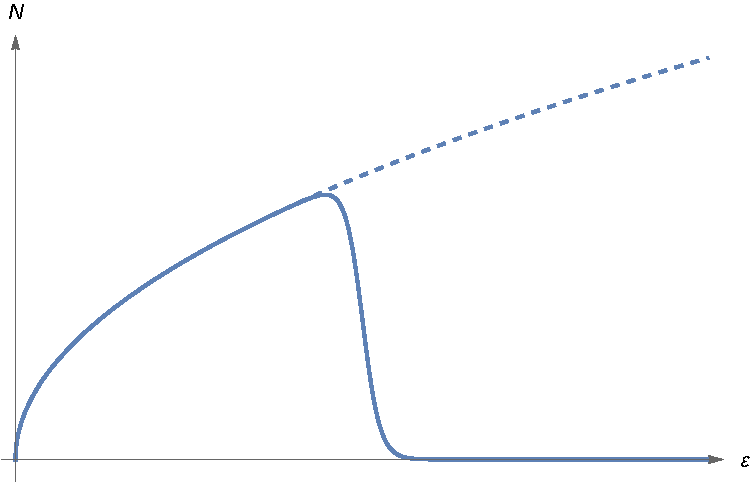
\includegraphics[width=0.42\textwidth]{fig/LowTempNum.pdf}}\qquad
    \subfigure[低温情形]{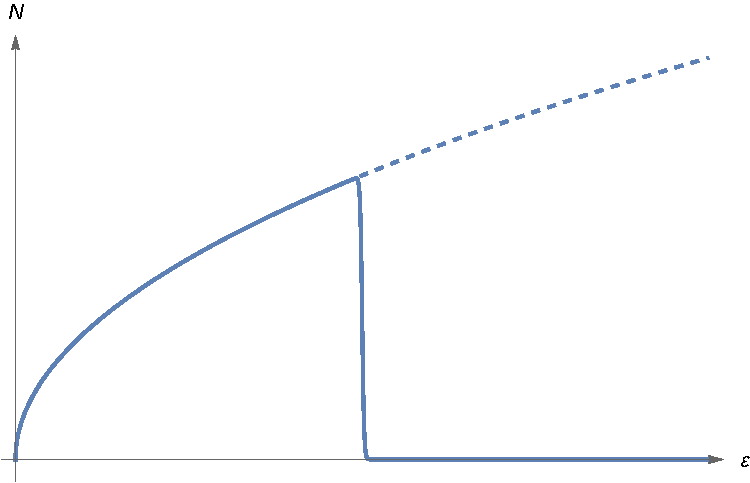
\includegraphics[width=0.42\textwidth]{fig/HighTempNum.pdf}}
    \caption{不同能级的粒子总数}
    \label{fig:fermi distribution times sqrte}
\end{figure}

记$x=\beta(\varepsilon-\mu)$,就有\begin{equation}
    f(x)'=\frac{e^x}{(e^x+1)^2}=\frac{1}{(1+e^x)(1-e^{-x})}
\end{equation}
利用巨正则系综中的结论\begin{equation}
    \beta p V =\ln \Xi =\sum_j g_j \ln (1+ e^{\beta (\mu-\varepsilon_j)}) \di \varepsilon
\end{equation}
对能级的求和可以化为对平动动能的积分\begin{equation}
    \ln \Xi =2 \int_0^\infty \rho(\varepsilon) \ln (1+e^{\beta (\mu-\varepsilon) })
\end{equation}
考虑到\begin{gather}
    \braket{N} = \sum_i \braket{n_i} =2 \int_{0}^{+\infty} \rho(\varepsilon) f(\varepsilon) \mathrm{d}\varepsilon\\
    \braket{E} =\sum_i \braket{n_i} \varepsilon_i =2\int_{0}^{+\infty} \rho(\varepsilon)f(\varepsilon) \varepsilon\mathrm{d}\varepsilon
\end{gather}

前面我们已经给出了\begin{equation}
    \rho(\varepsilon) \di\varepsilon =\frac{2\pi V}{h^3} (2m)^{3/2} \varepsilon^{1/2}\di \varepsilon
\end{equation}
\subsection{0K的情形} % (fold)
\label{sub:0K的情形}
这个时候电子只会占据$0\sim \mu_0$的能级,\begin{equation}
    f(\varepsilon)=\begin{cases}
        1 & \varepsilon <\mu_0\\
        0 & \varepsilon>\mu_0
    \end{cases}
\end{equation}
于是我们就有\begin{equation}
    \braket{N}=\int_0^{\mu_0} \frac{4\pi V }{h^3} (2m)^{3/2} \varepsilon^{1/2}\di \varepsilon =\frac{8\pi V}{3h^3} (2m)^{3/2} \mu_0^{3/2} \label{equ:N with E fermi}
\end{equation}
\begin{definition}
    我们称$T_F$满足\begin{equation}
        \mu_0 =k_B T_F
    \end{equation}
    为费米温度\index{费米温度}。
\end{definition}

\begin{example}
    常温下铜的密度为8.960g/cm³,尝试求铜的费米能级和费米温度。
\end{example}
\begin{solution}
    由式\eqref{equ:N with E fermi}可以得到\begin{equation}
        \mu_0 =(\frac{3h^3 \braket{N}}{8\pi V})^{2/3}/2m =1.0602\times 10^{-17} \mathrm{J}
    \end{equation}
    其费米温度为\begin{equation}
        T_F =\mu_F/k_B=7.68\times 10^5 \mathrm{K}
    \end{equation}
\end{solution}

平均能量满足\begin{equation}
    \begin{aligned}
        \braket{E} &= \int_0^{\mu_0} \frac{4\pi V}{h^3} (2m)^{2/3} \varepsilon^{3/2} \di \varepsilon\\
        &=\frac{2}{5} \frac{4\pi V}{h^3} (2m)^{2/3} \mu_0^{5/2}\\
        &=\frac{3}{5} \braket{N}\mu_0 =\frac{3}{5} \braket{N} k_B T_F
    \end{aligned}
\end{equation}
% subsection 0K的情形 (end)
\subsection{非0K的情形} % (fold)
\label{sub:非0K的情形}
一般地,我们有\begin{equation}
    \braket{E}= 2\int_{0}^{+\infty} \rho(\varepsilon) \varepsilon f(\varepsilon)
    \di \varepsilon 
\end{equation}
我们记\begin{equation}
    \varphi(\varepsilon) =2\int_0^\varepsilon \rho(\varepsilon') \varepsilon' \di \varepsilon'
\end{equation}
则$\displaystyle \di \varphi(\varepsilon) =\rho(\varepsilon) \varepsilon \di \varepsilon$,于是我们就有
\begin{equation}
    \begin{aligned}
        \braket{E}& =\int_0^\infty f(\varepsilon) \di \varphi(\varepsilon)\\
        &=\left. f(\varepsilon) \rho(\varepsilon) \right|_0^\infty -\int_{0}^{+\infty}\varphi(\varepsilon)f'(\varepsilon) \mathrm{d}\varepsilon
    \end{aligned}
\end{equation}
因为$\varepsilon\to+\infty$的时候和$\varepsilon\to 0$的时候$f(\varepsilon)\varphi(\varepsilon)$均趋于0,所以\begin{equation}
    \braket{E} = -\int_{0}^{+\infty}\varphi(\varepsilon)f'(\varepsilon) \mathrm{d}\varepsilon
\end{equation}
考虑到\begin{equation}
    f(\varepsilon)'=-\frac{\beta e^{\beta(\varepsilon-\mu)}}{(1+e^{\beta(\varepsilon-\mu)})^2}
\end{equation}
其大致图像为
\begin{figure}[h]
       \centering
       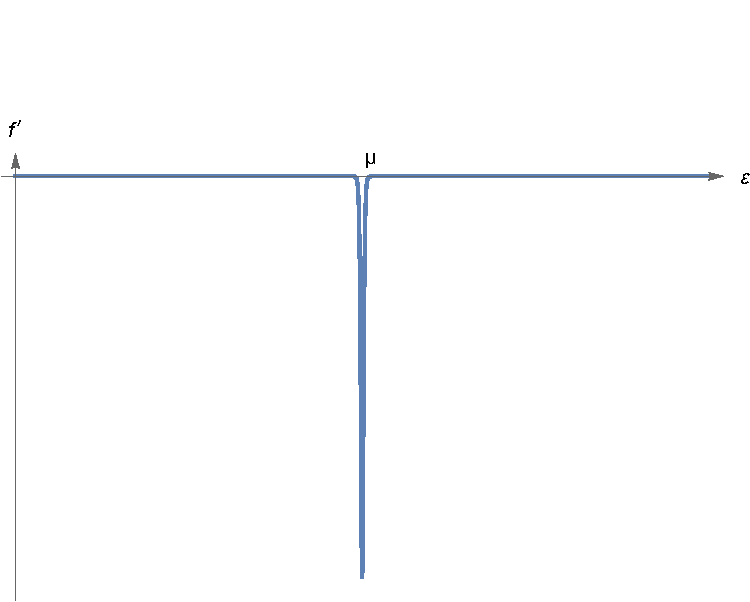
\includegraphics[width=0.5\textwidth]{fig/fermiD.pdf}
       \caption{$f'(\varepsilon)$函数}
       \label{fig:Dfermidistribution}
\end{figure}

所以\begin{equation}
    \braket{E} = -\int_{0}^{+\infty}\varphi(\varepsilon)f'(\varepsilon) \mathrm{d}\varepsilon \approx  -\int_{-\infty}^{+\infty}\varphi(\varepsilon)f'(\varepsilon) \mathrm{d}\varepsilon 
\end{equation}

我们将$\varphi(\varepsilon)$在$\varepsilon=\mu$的附近展开,因此就有\begin{equation}
    \varphi=\sum_{m=0}^\infty\left. \frac{\varphi^{(m)}(\varepsilon)}{m!}\right|_{\varepsilon=\mu}(\varepsilon-\mu)^m,\quad m=0,2,4,\cdots
\end{equation}

$m$取偶数是因为$f'(\varepsilon)$关于$\varepsilon-\mu$对称,因此奇数次项的积分为零。所以\begin{equation}
    \braket{E} =\sum_{m=0}^{\infty} \frac{\varphi^{(m)}(\mu)}{m!} \int_{-\infty}^{+\infty}(\varepsilon-\mu)^m [-f'(\varepsilon)] \mathrm{d}\varepsilon
\end{equation}
记$x=\beta(\varepsilon-\mu)$,我们记\begin{equation}
    L_m(x) = \int_{-\infty}^{+\infty}x^m/\beta^m [-f'(x)] \mathrm{d}\varepsilon=\frac{1}{\beta^m} \int_{-\infty}^{+\infty}\frac{x^m }{(1+e^x)(1+e^{-x})}\mathrm{d}\varepsilon 
\end{equation}
其中\[L_0 =1, \quad L_2=\frac{\pi^2}{3} (kT)^2,\quad L_4 =\frac{7\pi^4}{15} (kT)^4 \]
所以\begin{equation}
    \braket{E} =\sum_{m=0}^{\infty}L_m \frac{\varphi^{(m)}(\mu)}{m!}
\end{equation}

现在关键的问题是这个时候的$\mu$,为了求解这个$\mu$,我们首先求解$\braket{N}$,注意到\begin{equation}
    \braket{N} = 2  \int_{0}^{+\infty} \rho(\varepsilon) f(\varepsilon)\mathrm{d}\varepsilon 
\end{equation}
类似地,记$g(\varepsilon)=2\int_0^\varepsilon \di \varepsilon' \rho(\varepsilon')$,于是就有\begin{equation}
    \braket{N} =\sum_{m=0}^{+\infty} L_m\frac{g^{(m)}(\mu)}{m!}
\end{equation}
其中\[g(\varepsilon) = \frac{8\pi V}{3h^3} (2m)^{3/2} \varepsilon^{3/2},\quad g^{(2)} (\varepsilon) =\frac{2\pi V}{h^3} (2m)^{3/2} \varepsilon^{-1/2},g^{(4)}(\varepsilon)=\frac{3\pi V}{2h^3} (2m)^{3/2}\varepsilon^{-5/2}\]

所以\begin{equation}
    \begin{aligned}
        \braket{N}&=\frac{8\pi V}{3h^3}(2m)^{3/2}  \mu^{3/2} +\frac{\pi V}{h^3}(2m)^{3/2} \mu^{-1/2} +\frac{\pi V}{16h^3} \mu^{-5/2} +\cdots\\
        &= \frac{8\pi V}{3h^3}(2m)^{3/2}  \mu^{3/2}\left[1+\frac
        {\pi^2}{8} \left(\frac{kT}{\mu}\right)^2+o\left(\frac{kT}{\mu}\right)^4\right]
    \end{aligned}
\end{equation}
由于$N$不会随着温度变化而变化,所以当$T=0$的时候\begin{equation}
    \braket{N} = \frac{8\pi V}{3h^3}(2m)^{3/2}  \mu_0^{3/2}
\end{equation}
所以\begin{equation}
    \mu=\mu_0\left[1+\frac
        {\pi^2}{8} \left(\frac{kT}{\mu_0}\right)^2+o\left(\frac{kT}{\mu_0}\right)^4\right]^{-2/3}
\end{equation}
当$T$比较小的时候,就有\begin{equation}
    \mu=\mu_0\left[1-\frac
        {\pi^2}{12} \left(\frac{kT}{\mu_0}\right)^2 +o\left(\frac{kT}{\mu_0}\right)^4\right]
\end{equation}
也即:随着温度的升高,化学势略有降低,但是下降的不多。

现在我们完成了$\mu$的求解,于是就有\begin{equation} 
    \braket{E} =\sum_{m=0}^{\infty}L_m \frac{\varphi^{(m)}(\mu)}{m!}
\end{equation}
因为\begin{equation}
    \begin{gathered}
        \varphi(\varepsilon)=\frac{4\pi V}{h^3} (2m)^{3/2}\int_0^\varepsilon {\varepsilon'}^{3/2} \mathrm{d}\varepsilon'= \frac{8\pi V}{5h^3} (2m)^{3/2} \varepsilon^{5/2}\\
        \varphi^{(2)}(\varepsilon)= \frac{6\pi V}{h^3} (2m)^{3/2} \varepsilon^{1/2},\quad
        \varphi^{(4)}(\varepsilon)= \frac{9\pi V}{2h^3} (2m)^{3/2} \varepsilon^{-3/2}
    \end{gathered}
\end{equation}
所以\begin{equation}
    \begin{aligned}
        \braket{E} &=\frac{8\pi V}{5h^3}(2m)^{3/2}  \mu^{5/2} +\frac{3\pi V}{h^3}(2m)^{3/2} \mu^{1/2} \frac{\pi^2}{3}(kT)^2+\frac{3\pi V}{16h^3} \mu^{-3/2} \frac{7\pi^4}{15}(kT)^2+\cdots\\
        &= \frac{8\pi V}{5h^3}(2m)^{3/2}  \mu^{5/2}\left[1+\frac
        {5\pi^2}{8} \left(\frac{kT}{\mu}\right)^2+o\left(\frac{kT}{\mu}\right)^4\right]\\
        &= \frac{8\pi V}{5h^3}(2m)^{3/2}  \mu_0^{5/2}\left[1-\frac
        {5\pi^2}{24} \left(\frac{kT}{\mu_0}\right)^2+o\left(\frac{kT}{\mu_0}\right)^4\right] \left[1+\frac{5\pi^2}{8}\left(\frac{kT}{\mu_0}\right)^2+o\left(\frac{kT}{\mu_0}\right)^4\right]\\
        & = \frac{8\pi V}{5h^3}(2m)^{3/2}  \mu_0^{5/2}\left[1+\frac
        {5\pi^2}{12} \left(\frac{kT}{\mu_0}\right)^2+o\left(\frac{kT}{\mu_0}\right)^4\right]\\
        & = \braket{E}_0 \left[1+\frac
        {5\pi^2}{12} \left(\frac{kT}{\mu_0}\right)^2+o\left(\frac{kT}{\mu_0}\right)^4\right]\\
        & =\frac{3}{5} Nk_B T_F \left[1+\frac
        {5\pi^2}{12} \left(\frac{kT}{\mu_0}\right)^2+o\left(\frac{kT}{\mu_0}\right)^4\right]
    \end{aligned}
\end{equation}

由此可以得到系统的热容为\begin{equation}
    C_V= \diffp*{{\braket{E}}}{T}{\, V} = \frac{3}{5} Nk_B T_F \frac{\pi^2}{12} \frac{2T}{T_F^2} +o(T^3) =\frac{\pi^2}{2} Nk_B \frac{T}{T_F}
\end{equation}
根据式\eqref{equ:C_V in crystal},晶体由晶格振动带来的热容为\begin{equation}
    C_V =\frac{12}{5}\pi^4 N K_B \left(\frac{T}{\theta_D}\right)^3 \propto T^3
\end{equation}
因为$T_F$很大,所以温度较高的时候,自由电子气的热容相比于晶格振动的热容要小很多。但是极低温度下,晶格热容$C_V \propto T^3$,此时自由电子气热容占主导。

% subsection 非0K的情形 (end)
% section 统计分析 (end)
\section{习题} % (fold)
\label{sec:习题8}

% section 习题 (end)
% chapter 自由电子气 (end)
%---------------------------------------------------------------------------